\section{Data Exploration}

The first step in understanding the insect data is to investigate the yearly abundance. \Cref{fig:total-count} reveals that the data (all traps combined) contains three dominating species: \textit{Vanessa atalanta}, \textit{Inachis io} and \textit{Vanessa cardui}. While \textit{V. atalanta} is recorded consistently in recent years, \textit{V. cardui} and \textit{I. io} show high variation. Most prominently, \textit{I. io} shows pronounced outbreaks in 1985, 2002 and 2011.

\begin{figure}[H]
	\centering
	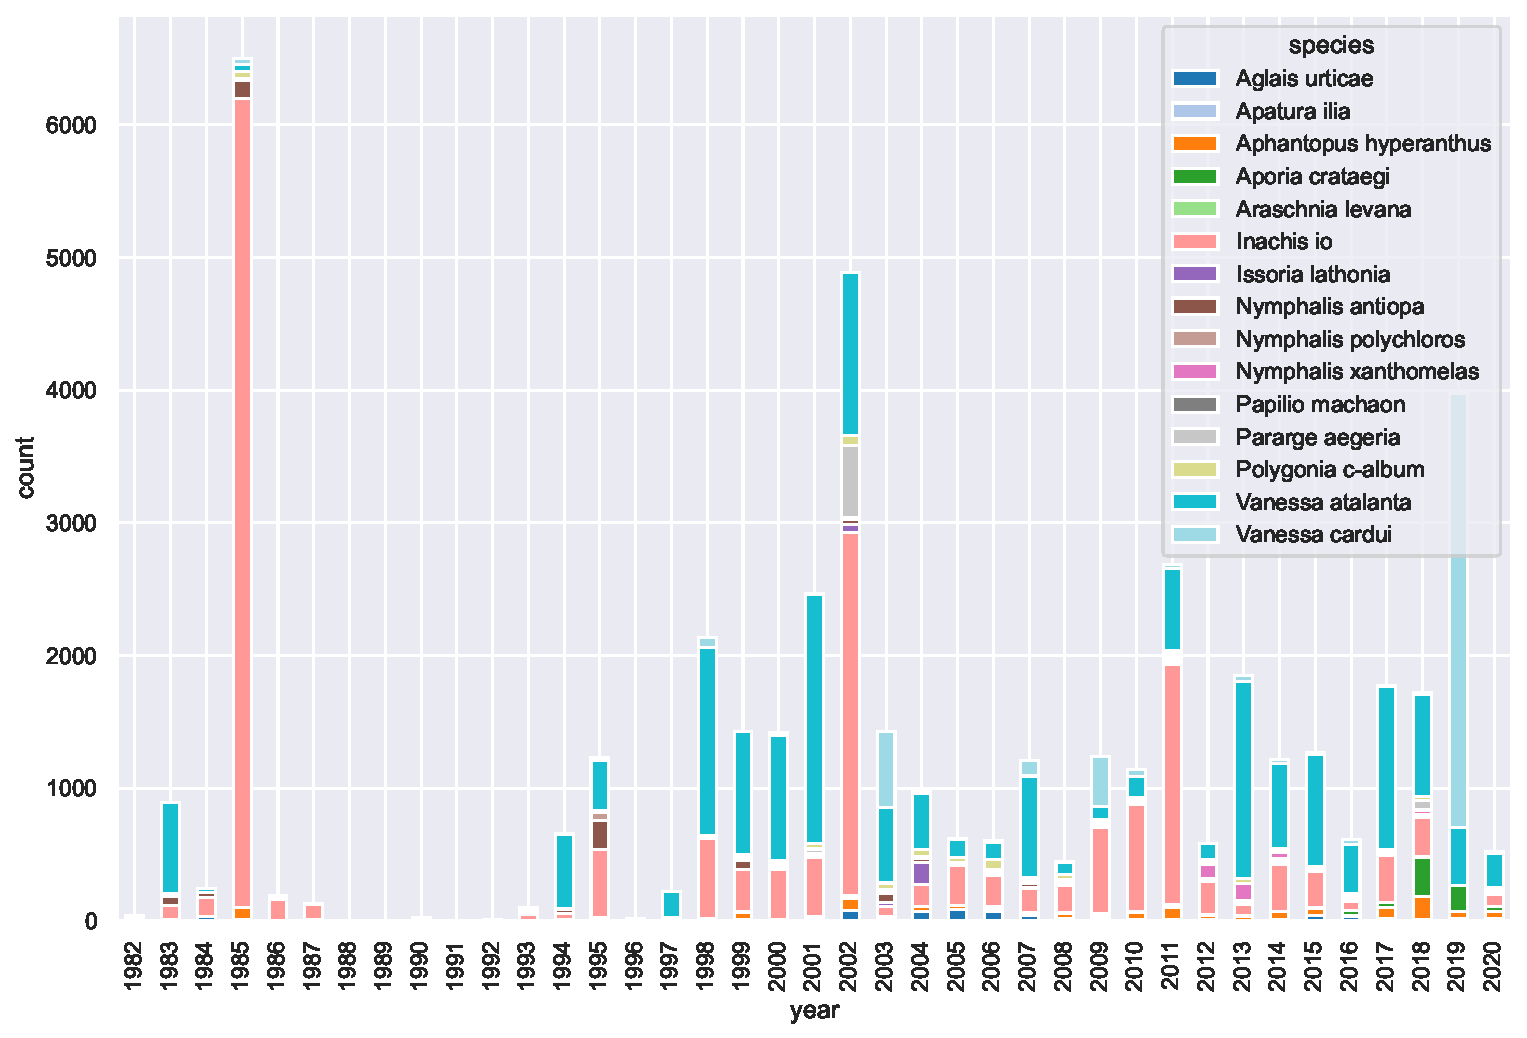
\includegraphics[width=0.9\linewidth]{figs/total-count_per_year_per_species}
	\caption{The total count per year split into single species (\href{https://github.com/gtlab-barcelona/Robert/blob/main/data-exploration_first-last/figs/total-count_per_year_per_species.pdf}{image link}).}
	\label{fig:total-count}
\end{figure}

\subsection{Missing Values}\label{sec:nans}

The dataset has a high number of missing values in early years, with considerable \enquote{improvement} from 1998 onwards. Contrary to expectations, the number of missing values in temperature and insect count is not equal. Apparently there have been days in which insect count was monitored, but temperature was not recorded, and vice versa.
Consequently, in order to yield more consistent results, the data analysis is constrained to the time period from 1998 to 2020.

\begin{figure}[H]
	\centering
	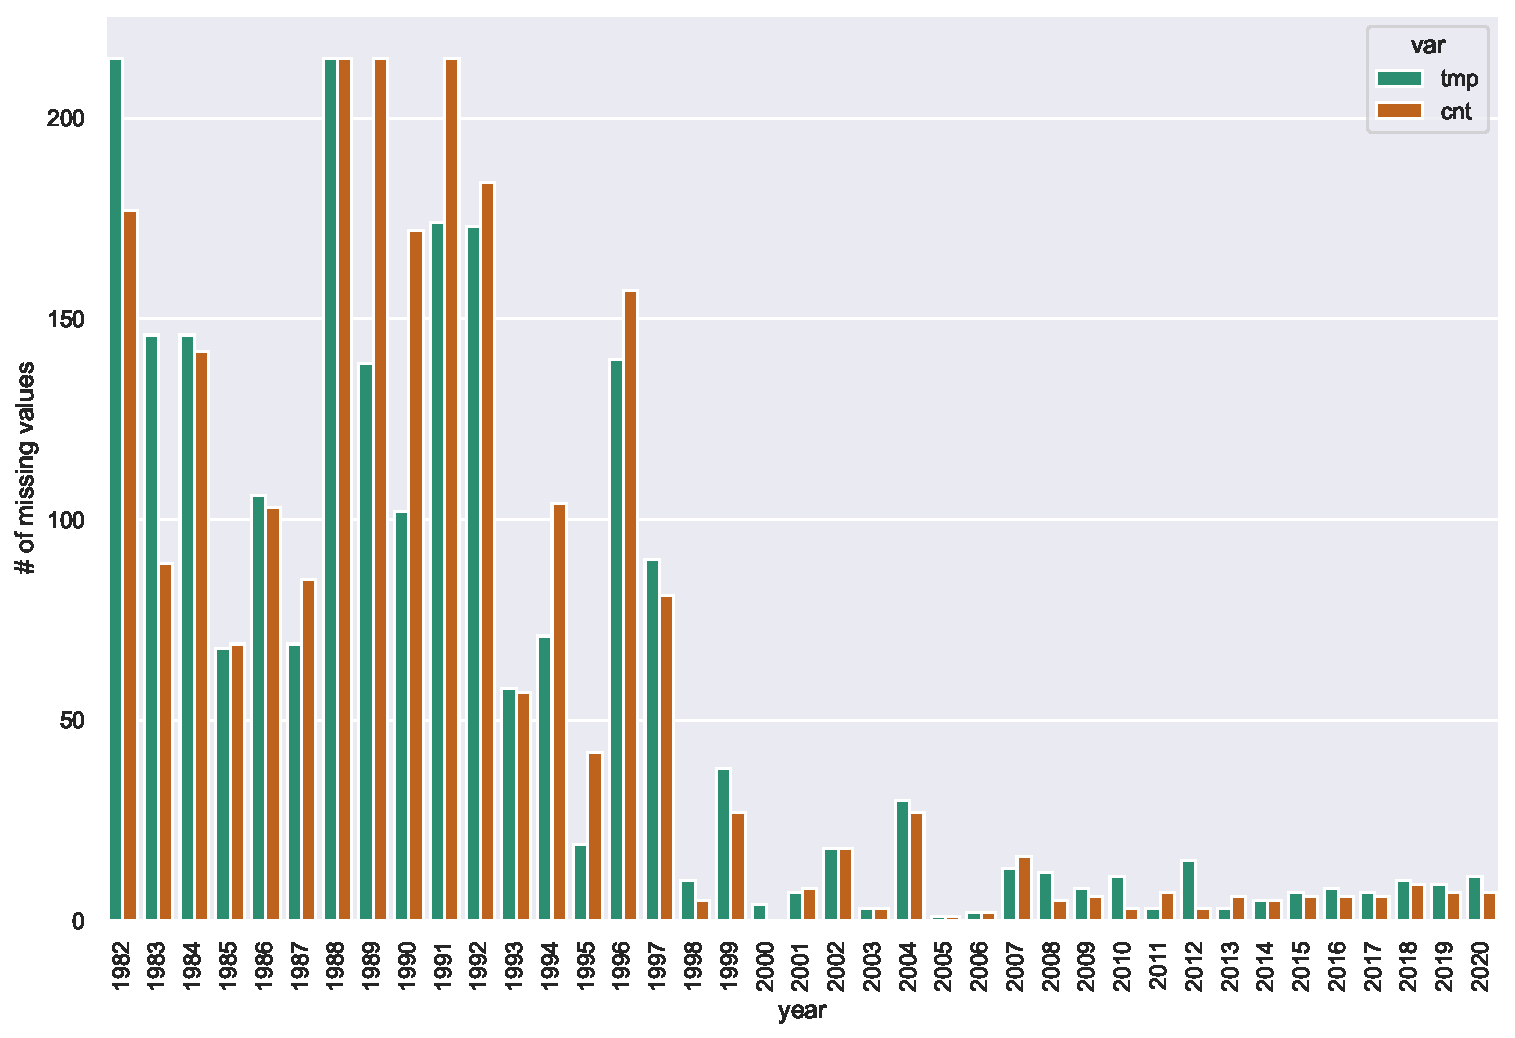
\includegraphics[width=0.9\linewidth]{figs/nans_per-year}
	\caption{Number of missing values in temperature (\textit{tmp}; green) and insect count (\textit{cnt}, orange) per year (\href{https://github.com/gtlab-barcelona/Robert/blob/main/data-exploration_first-last/figs/missing-data/nans_per-year.pdf}{image link}).}
	\label{fig:nans-per-year}
\end{figure}